\subsection{Introduction}

Small molecules are excellent tools for probing biological functions and continue to be the cornerstone of pharmaceutical companies. Synthetic chemical compounds present a complex structural code that, for the most part, has not been explored by the principles of natural evolution. Many pharmacological compounds are imperfect human inventions with sub-optimal bioactivities that lack a clear connection to their chemical structure. Often, the only way to approach the biological characterization of a compound is to assume it will have comparable bioactivities to compounds with similar chemical properties. The so-called ‘similarity principle’ has been the driving force of drug discovery efforts\cite{kumar_advances_2018}, and the measurement of compound similarities lays behind most of the approaches used to explore the vast drug-like chemical space (estimated in the range of 10\textsuperscript{33}-10\textsuperscript{66} molecules\cite{polishchuk_estimation_2013, bohacek_art_1996}). To assess such similarities, molecules are usually characterized using numerical fingerprints or descriptors\cite{cereto-massague_molecular_2015}, which encapsulate their main topological and physicochemical properties representing them in a format amenable for computational applications (e.g. QSAR\cite{yang_concepts_2022}).

In the last years, the extensive gathering and release of bioactivity data have shown that the similarity principle applies beyond standard chemical features, reaching to functional properties. For instance, small molecules that show similar sensitivity profiles across human tumor cell-lines or drugs that cause comparable side effects in patients tend to share mechanisms of action (MoA), even when they are structurally dissimilar\cite{holbeck_analysis_2010, seashore-ludlow_harnessing_2015, campillos_drug_2008}. Thus, bioactivity similarities offer an alternative means to functionally characterize small molecules, potentially providing insights closer to clinical observations and surpassing what is expected from merely inspecting chemical analogues\cite{petrone_rethinking_2012}.

%%%%%%%%%%%%%%%%
%%% FIGURE 1 %%%
%%%%%%%%%%%%%%%%


\begin{figure}[t!]
  \centering
  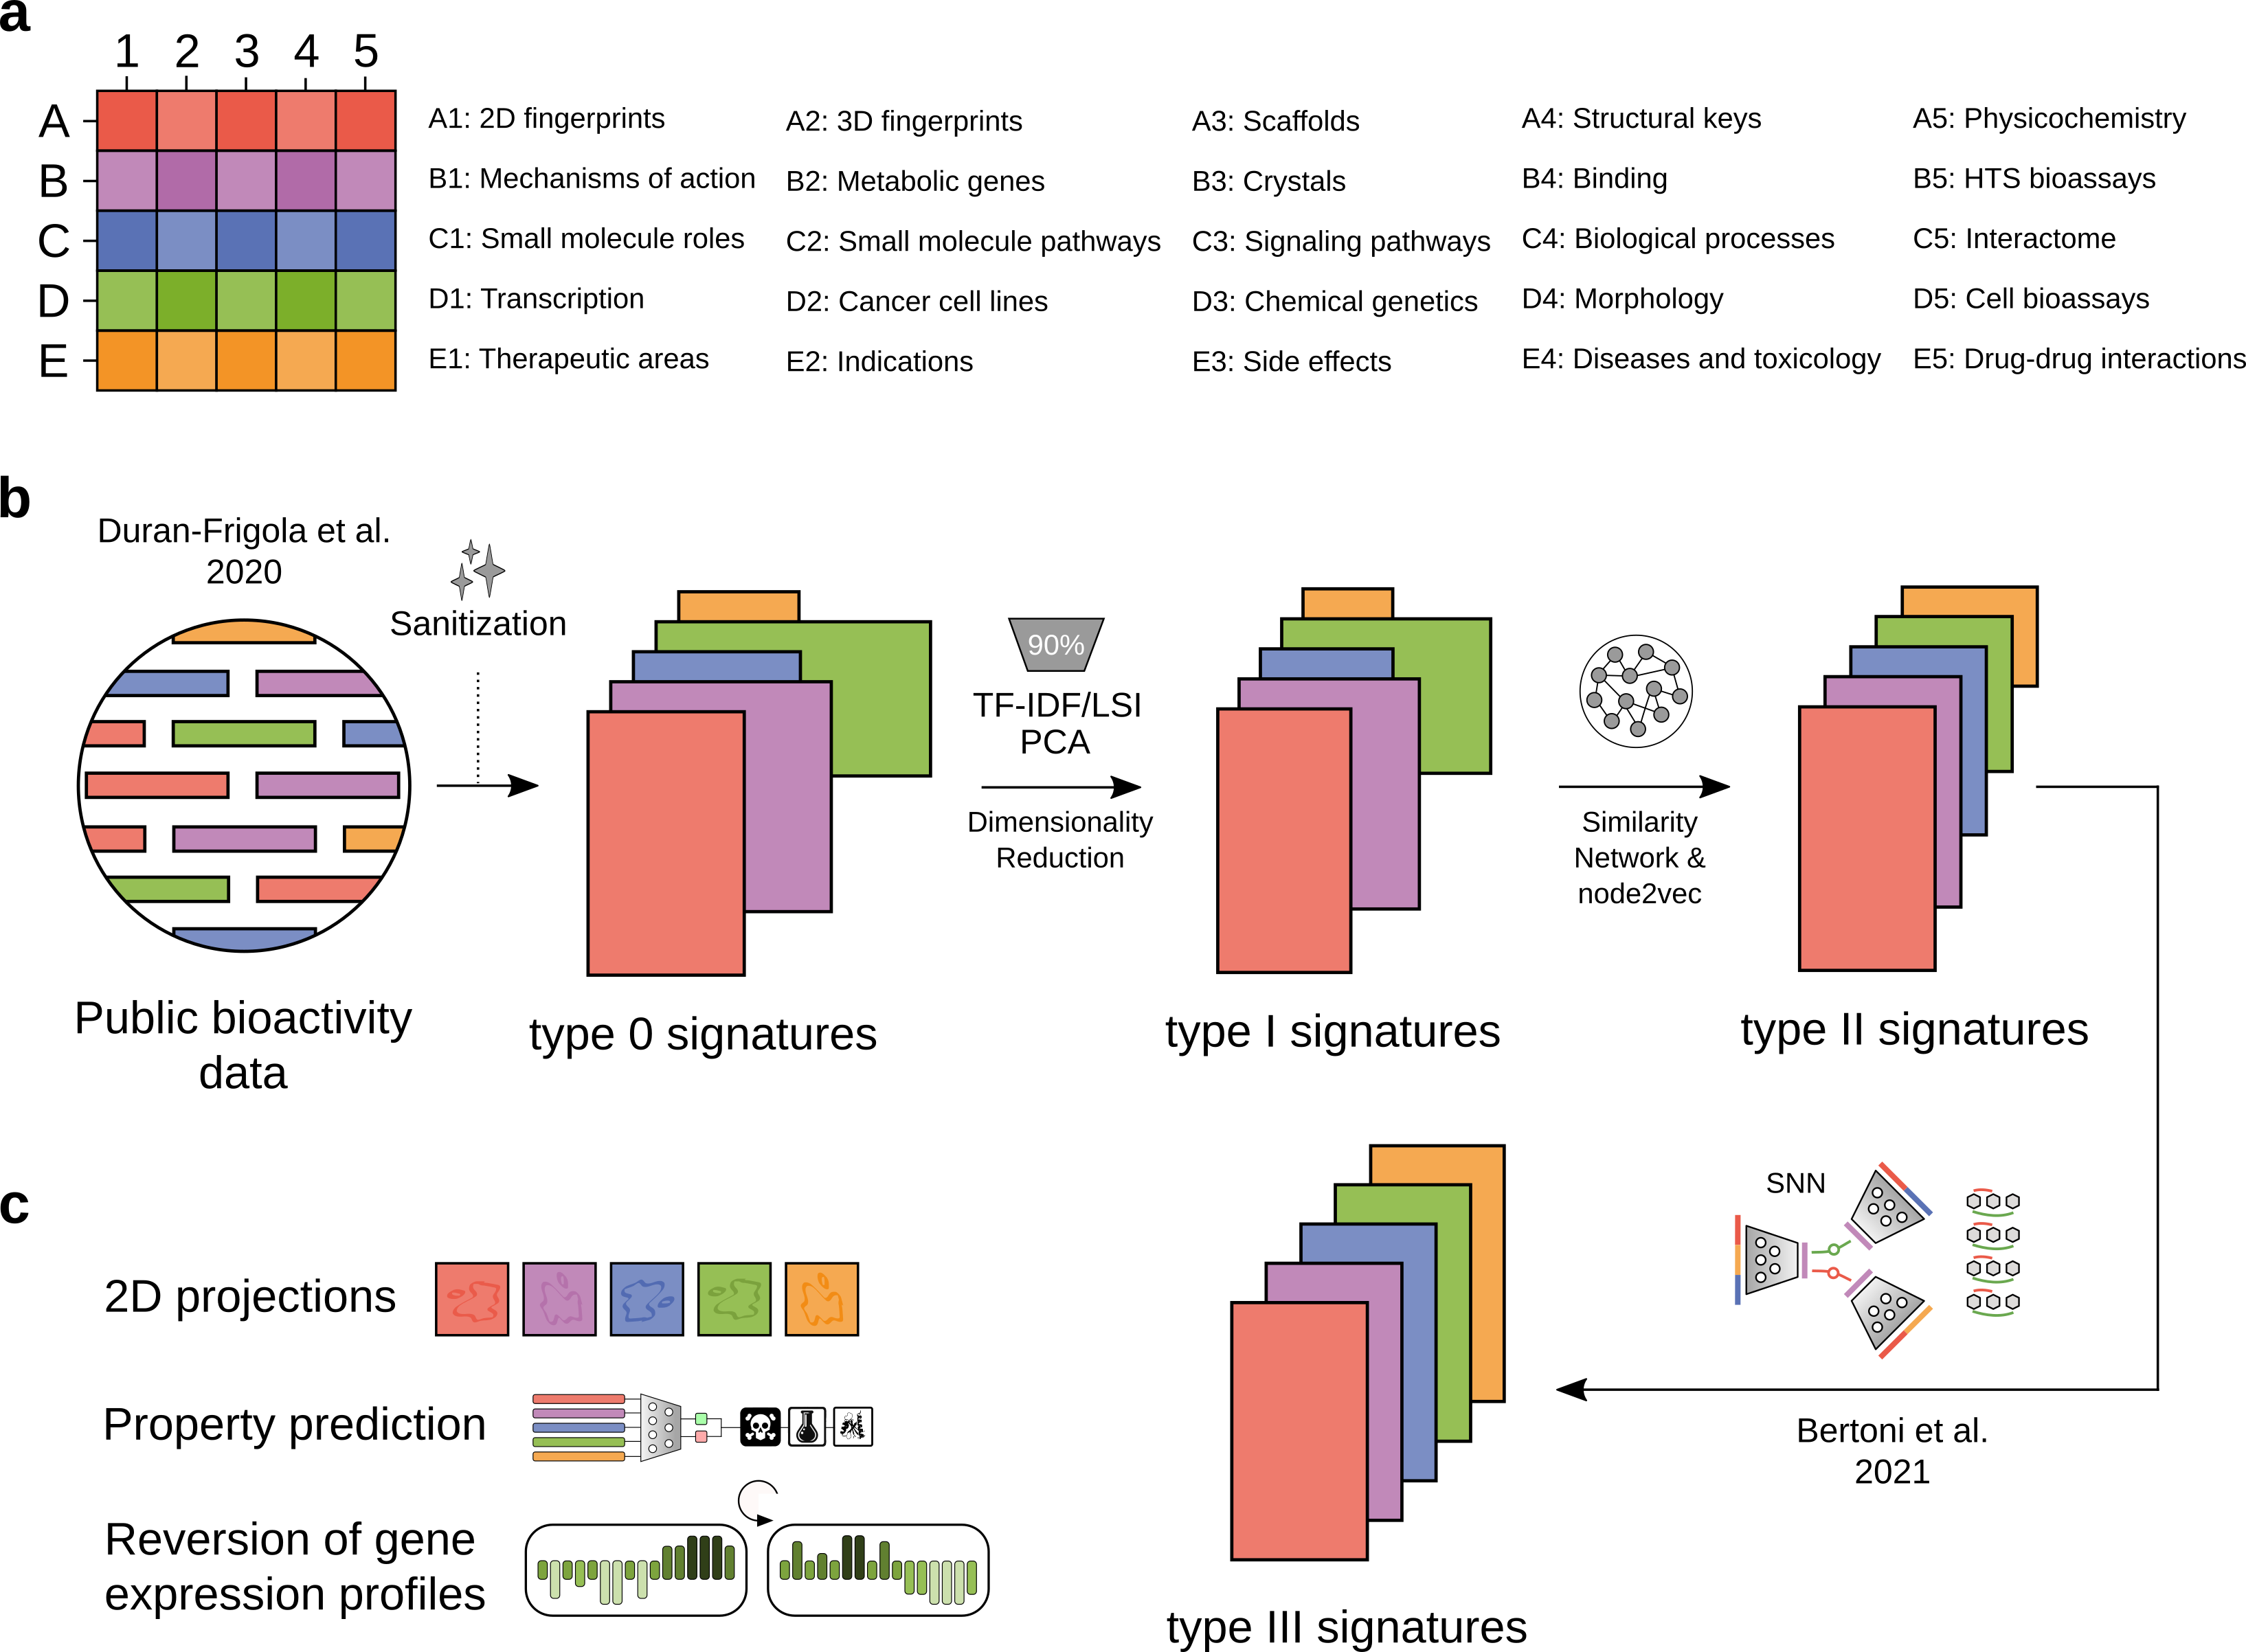
\includegraphics[width=\linewidth]{figures/Protocols/Main/CC.png}
  \caption{
    \textbf{CC Overview.} 
    \textbf{a)} Organization of the 25 CC spaces.
    \textbf{b)} Computational pipeline to build the CC and procedure to integrate bioactivity data in the CC universe. In brief, bioactivity data is sanitized (type 0 signatures), compressed (type I signatures), harmonized (type II signatures) and integrated with all the other data within the CC (type III signatures).
    \textbf{c)} Compound signatures are used in a variety of tasks, such as the characterization and visualization of large small molecule libraries, the prediction of multiple properties (e.g. toxicity, physicochemical properties, protein binding, etc.) and the reversion of gene expression profiles associated with specific disease states, among many others. 
  }
  \rule[0ex]{\textwidth}{0.5pt}
  \vspace{-5mm}
  \label{Protocols_Fig1}
\end{figure}



\phantomsection
\subsubsection{The Chemical Checker}

We recently developed the Chemical Checker (CC, Fig \ref{Protocols_Fig1}a), the largest collection to date of processed, harmonized and integrated bioactivity signatures for over 1 million compounds, whose biological effects had been experimentally determined\cite{duran-frigola_extending_2020}. Following the way in which we understand drug action, we organized data in 25 bioactivity spaces grouped in 5 levels of increasing biological complexity: from physicochemical and structural properties of small molecules (A) to the clinical effects they exert in human patients (E). In between, we collect the set of biological targets they bind (B), the perturbations they trigger in biological pathways (C) and the phenotypic effects they induce in cell-based assays (D). Unfortunately, bioactivity data become scarcer and more difficult to obtain as biological complexity increases (i.e. we have direct protein-binding data for \textasciitilde630k small molecules but only \textasciitilde6k compounds are annotated with clinical indications), meaning that bioactivity information remains limited for poorly characterized compounds. Indeed, out of the 10\textsuperscript{33}-10\textsuperscript{66} synthetically accessible drug-like molecules\cite{polishchuk_estimation_2013, bohacek_art_1996}, only a tiny fraction has experimentally measured chemical properties or bioactivities reported in public databases (i.e. \textasciitilde120M in PubChem and \textasciitilde2.4M in ChEMBL as of October 2024). To address this problem, we developed a collection of deep neural networks to infer CC bioactivity signatures for any compound of interest\cite{bertoni_bioactivity_2021, comajuncosa-creus_stereochemically-aware_2024}, based on the observation that the different bioactivity spaces are not completely orthogonal, and thus similarities of a given bioactivity type (e.g. targets) can be transferred to other data kinds (e.g. therapeutic indications). Moreover, we showed that the inferred bioactivity signatures are useful to navigate the chemical space in a biologically relevant manner and improve the performance of biophysics and physiology activity prediction activities with respect to chemistry-only based classifiers\cite{bertoni_bioactivity_2021}. In general, we believe that bioactivity signatures associated to small molecules have the power to reintroduce the biological complexity at the early stages of the drug discovery process, overcoming some of the problems associated with target-based approaches. For instance, using CC signatures, we were able to identify three compounds able to revert transcriptional signatures related to Alzheimer’s disease \textit{in vitro} and \textit{in vivo}\cite{pauls_identification_2021}. Moreover, using CRISPR-Cas9 and shRNA perturbation experiments as templates, we also identified several small molecules that mimicked the phenotypic effects of biodrugs (e.g. daclizumab, ustekizumab, cetuximab, etc.), often through a different MoA that did not directly modulate the activity of their primary targets (e.g. IL-2R, IL-12 and EGFR)\cite{duran-frigola_extending_2020}, and targeted cancer proteins though to be undruggable\cite{bertoni_bioactivity_2021}.


The original 25 CC bioactivity spaces (Fig \ref{Protocols_Fig1}a) comprise data retrieved from publicly available databases at the time that were processed through a unified data curation and integration pipeline. Compound bioactivities are expressed in a vector-like format (i.e. signatures) and organized in increasing levels of abstraction: from raw data accounting for explicit knowledge (type 0 signatures) to inferred representations leveraging known bioactivity patterns (type III signatures). However, in the last years, new large-scale assays to capture biological responses to small molecule perturbations, and more efficient computational strategies to process them, are constantly appearing\cite{anglada-girotto_combining_2022, mitchell_proteome-wide_2023, offensperger_large-scale_2024}. Besides, there is an ever-growing number of laboratories and biotechnological companies that have their own in-house data and want to leverage it together with the bulk of known bioactivity information. Thus, in this manuscript, we present the complete computational protocol to generate novel bioactivity spaces and signatures, describing the main steps needed to leverage diverse bioactivity data with the Chemical Checker (type 0, type I, type II and type III signatures) using the predefined data curation and integration pipeline.

\phantomsection
\subsubsection{Overview of the Chemical Checker data integration pipeline}
\label{Overview of the Chemical Checker data integration pipeline}

The main input for the CC integration pipeline is a bioactivity data matrix encompassing compounds (rows, e.g. InChIKeys) and biological features (columns, unique strings: e.g. protein targets (B4), mechanisms of action (B1), clinical side effects (E3), etc.). Data might be categorical (e.g. binary), discrete or continuous.

\paragraph{-- Type 0 signatures --} \leavevmode

The very first step in the CC processing framework is to produce a sufficiently-curated and sanitized version of the raw bioactivity data (Fig \ref{Protocols_Fig1}b). To achieve this, features (columns) that are extremely sparse (i.e. occurring in few rows) or too prevalent (i.e. occurring in almost all rows) are removed from the matrix and those compounds (rows) showing no feature occurrences are discarded. In addition, not-available (NA) and infinite values are processed (median-imputed and max/min values, respectively) and low-Shannon entropy features are trimmed if the maximum number of allowed features is surpassed. Overall, type 0 signatures represent explicit knowledge, allowing direct interpretation while having variable dimensionality. 

\paragraph{-- Type I signatures --} \leavevmode

The second processing step implies a mild compression of type 0 signatures typically retaining 90\% of the original variance and thereby reducing the number of vector dimensions (Fig \ref{Protocols_Fig1}b). For discrete data, a term frequency–inverse document frequency (TF–IDF) transformation is used to weight features (columns) according to their information retrieval (i.e. more frequent features are less informative and thus become underweighted). After that, a Latent Semantic Indexing (LSI) dimensionality reduction technique is applied to the TF–IDF transformed data and LSI components explaining 90\% of the original variance are kept to build type I signatures. For continuous data, the matrix is first scaled column-wise (median 0, median absolute deviation 1 and capped at ±10) and then processed through a PCA. Analogously to discrete data, PCA components explaining 90\% of the original variance are kept to build type I signatures. Overall, type I signatures are better optimized for compound similarity calculations, although they no longer represent explicit knowledge and still have variable dimensionality.  

\paragraph{-- Type II signatures --} \leavevmode

The main purpose of type II signatures is to retain similarities at type I signature level while harmonizing the length of vectors among CC spaces (i.e. converting signatures of variable dimensionalities to 128-length vectors, Fig \ref{Protocols_Fig1}b). First, a similarity network is built considering nearest neighbors (NN) at type I signature level for each compound (small molecules represent the nodes in the graph and their similarities are the edges). Then, the node2vec algorithm is run to create an embedding for each molecule (node), encoding intrinsic relationships within the similarity graph. In this way and, although not directly interpretable, type II signatures capture explicit and implicit similarities in the data. Additionally, the fixed length (128) makes the concatenation of descriptors across bioactivity spaces cost-effective, while ensuring that each bioactivity space contributes equally to the overall representation.  


\paragraph{-- Type III signatures --} \leavevmode


The last step in the processing framework is the generation of type III signatures for the input compounds and for all the molecules in the CC, which capture and infer the similarity of the data at type I signature level (Fig \ref{Protocols_Fig1}b). The approach is based on the observation that different CC spaces are not completely orthogonal and may show correlation to some extent. In short, for each CC space, a Siamese Neural Network (SNN) is trained over 10 million triplets of compounds (anchor, positive and negative molecules sampled at type I signature level) representing these input molecules by concatenating all available type II signatures. After being validated, the SNN generates novel signatures (type III) that retain the observed similarities at type I signature level and accounts for compound data present in every other bioactivity space of the CC, allowing the inference of a bioactivity signature even in the absence of data for the molecule of interest. It is worth mentioning that the generation of type III signatures is usually the most computationally expensive step in the CC data integration pipeline, and strongly benefits from parallelization.

Since most properties and similarities at type III signature level are inferred, each of them comes together with a measure of confidence called ‘applicability’ (from 0 to 1). Applicability scores evaluate the distance to training-set signatures, the robustness of the predicted signatures and the expectancy a priori given the known data. For further details about signature inference and confidence score, we refer the reader to the original publication\cite{bertoni_bioactivity_2021}.

\paragraph{-- Additional remarks --} \leavevmode

The outlined pipeline includes numerous distinct steps, each possessing its own set of default options and parameters. While the user can modify the vast majority of parameters, the whole point of the computational pipeline –and where we put most emphasis– is in the full automation. In fact, the approach works end-to-end, and it is very robust to very different data shapes and types (sparse, long, wide, dense, etc.). Thus, we recommend to use the by default parameters, but give the possibility to the user to adapt them if new uses of the CC signatures might arise. For additional details on such parameters and further clarification of the mentioned steps we refer to the original publications\cite{duran-frigola_extending_2020, bertoni_bioactivity_2021} and our regularly maintained GitLab repository (\href{https://gitlabsbnb.irbbarcelona.org/packages}{https://gitlabsbnb.irbbarcelona.org/packages}). 

In addition, to monitor and evaluate data flow at each step of the CC integration pipeline, we have designed several analyses to assess the obtained results in a systematic manner. An exhaustive description of all benchmarking studies can be found in the \hyperref[Protocols_SupplementaryInformation]{Supplementary Information}. 

\phantomsection
\subsubsection{Building new Chemical Checker bioactivity spaces}
\label{Building_NEW_CC_BIOACTIVITY_SPACES}

To comprehensively illustrate the use of the protocol to build bioactivity spaces and signatures associated to small molecules, we adapt it to four distinct scenarios: i) introducing additional data into an existing CC bioactivity space (\textbf{B1.002} space), ii) creating a new version of an existing CC bioactivity space with a different strategy of input data processing (\textbf{D1.002} space), iii) creating a CC bioactivity space from a novel data type that fits the actual CC universe (i.e. human-derived data, \textbf{D6.001} space) and iv) creating a CC bioactivity space from a novel data type that does not fit the actual CC universe (i.e. measuring compound effects on bacterial species, \textbf{M1.001} space). The CC nomenclature to define the different bioactivity spaces first notes the space (i.e. A1-n, B1-n, etc) and then numbers the dataset or processing protocols used (i.e. 001, 002, etc).